\chapter{Premier pas vers SymPy}

Ce chapitre d’introduction présente la tournure d’esprit de la bibliothèque mathématique SymPy. Les 
autres chapitres de cette partie développent les notions de base de SymPy: effectuer des calculs 
numériques ou symboliques en analyse, opérer sur des vecteurs et des matrices, écrire des programmes, 
manipuler des listes de données, construire des graphiques, etc. Les parties suivantes de cet ouvrage 
approfondissent quelques branches des mathématiques dans lesquelles l’informatique fait preuve d’une 
grande efficacité.

\section{La bibliothèque SymPy}

\subsection{Le cas de la bibliothèque SymPy}

Dans un cas plus simple l'exemple 1.1 se formule beaucoup plus dans un outil comme SymPy est une bibliothèque de calcul formel elle est aussi un environnement pour 
l’apprentissage de l’algèbre, l’analyse, géométrie, combinatoire, cryptographie, mécanique 
classique et quantique pour le lycée et l’université mais aussi un environnement de 
développement et de recherche. SymPy  écrit entièrement en Python un langage de 
programmation facile à apprendre et adapté à l’apprentissage,  elle fourni aux étudiant 
\textit{SymPyGamma} une application web   notamment des primitives générales de traitement des 
expressions algébriques (développement, factorisation, …), des aides à l’organisation des objets 
mathématiques intervenant dans la résolution d’un problème ainsi qu’une assistance à la preuve. Il 
permet au professeur de préparer et de suivre le travail de l’élève. Différentes maquettes ont été 
développées et testées auprès d’élèves. Dans la plus récente, nous nous sommes attachés à explorer une 
nouvelle forme d’activité algébrique. Alors que le calcul en papier crayon et les logiciels standards 
considèrent  les expressions de façon isolée, l’environnement que nous développons organise en réseau 
les différentes expressions intervenant dans la résolution d’un problème. L’ordinateur peut facilement 
mettre à jour ce réseau quand l’utilisateur modifie certains de ses éléments. Il devient ainsi possible, 
pour aborder un problème générique, d’explorer facilement des cas particuliers et de conduire une 
généralisation. Les relations entre expressions algébriques sont mieux mises en évidence du fait de leur 
invariance dans les modifications du réseau. De façon très concise, Casyopée peut être défini
\subsection{Travaillez avec SymPy}
Pour utiliser Sage, il suffit d’un navigateur web tel que Firefox. Le plus simple dans un premier temps est de se connecter sur un serveur de calcul Sage public comme http://sagenb.org/. On a alors accès à une interface utilisateur riche constituée d’un « bloc-notes » (notebook en anglais) permettant d’éditer
et partager des feuilles de travail (worksheets, voir figure 1.2). De nombreuses universités et institutions mettent de tels serveurs à la disposition de leurs utilisateurs ; renseignez-vous autour de vous. Pour un usage plus intensif, on

installe généralement Sage sur sa propre machine 1 . On peut alors toujours
l’utiliser avec l’interface bloc-notes dans le navigateur web. Alternativement, on
peut l’utiliser en ligne de commande, comme une calculatrice (voir figure 1.3).
Les figures 1.4 et 1.5 illustrent pas à pas les étapes pour accéder à un serveur
Sage public et l’utiliser pour faire un calcul :


\subsubsection{SymPyGamma}
Est une interface onWeb marche avec un navigateur contient plusieurs catégorie liée de calcul, dynamique. L’Intérêt de cette outil qu'il est facilement partageable adapté pour l’enseignement et surtout l'auto-apprentissage

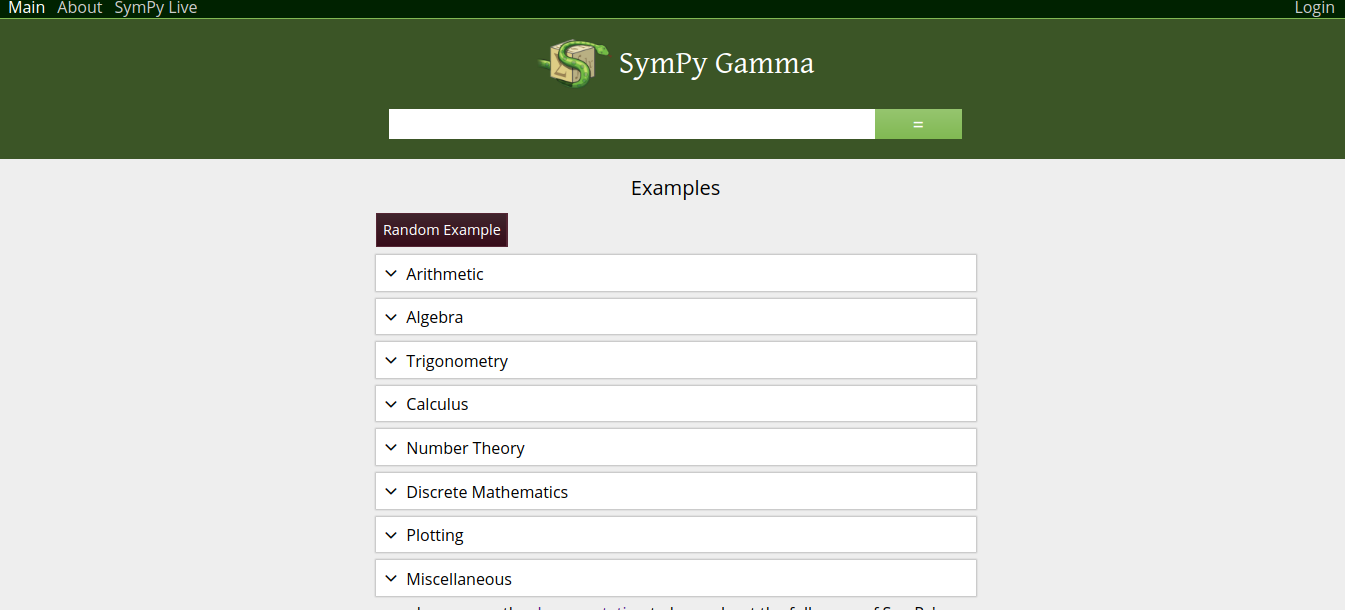
\includegraphics[scale=0.3]{../Pictures/sympyGammaMain.png} 

\subsubsection{SymPyLive}
SymPy Live est SymPy qui s'exécute sur Google App Engine. Ceci est juste un shell Python standard, avec les commandes suivantes exécutées par défaut
\section{SymPy comme calculatrice}
Contrairement à Sage[], Maple, Octave et les autres logiciel de calcul formel, SymPy, effectue des calculs directe numériques de deux manière différents en passant par la méthode, 
\subsection{Premier calculs}
\subsubsection{Variables Python}
Lorsque l’on veut conserver le résultat d’un calcul, on peut l’affecter à une
variable :

\subsubsection{Variables Symboliques}
Les objets mathématiques manipulés par SymPy sont symboliques ils sont représentés exactement loin de 
toute approximation numérique, SymPy permet une manipulation avec des expressions contenant
des variables, comme $x^{2} + zy^{3} + z^{2}$ ou encore $sin(x) - exp(x)$. Les variables symboliques
du mathématicien $x$, $y$, $z$ apparaissant dans ces expressions diffèrent, avec SymPy,
des variables du développeur $sin(2) = 0.9092974268256817$ que nous manipulons sous Python 
section précédente. 


\subsection{Structure de données dans SymPy}
Le moteur symbolique de SymPy tire parti de l'orientation des objets (notamment l'héritage) pour créer une base de code facilement extensible. Toutes les classes dérivent des fonctionnalités, telles que la possibilité de se comparer à d'autres objets, à partir de méthodes de la super-classe Basic. Les objets pouvant faire l'objet d'opérations algébriques acquièrent cette capacité grâce à un ensemble de méthodes d'une classe appelée Expr. Ces objets Expr peuvent être conservés dans des objets conteneur (qui contiennent également la sous-classe Expr) Mul, Add et Pow; les objets conteneur sont instanciés à l'aide de l'opérateur Python, tel que la fonction de surcharge, qui permet au constructeur de la classe conteneur d'être appelé chaque fois que l'opérateur binaire approprié est utilisé (* pour Mul, + pour Ajouter et $**$ pour Pow).
De cette manière, des objets supplémentaires peuvent être ajoutés en créant simplement une sous-classe qui hérite des fonctionnalités de la classe Expr. Ces sous-classes bénéficient gratuitement de certaines fonctionnalités, telles que la possibilité de comparer, de multiplier, d’ajouter, etc. Voici comment SymPy crée un environnement modifiable, maintenable, et donc facile à étendre. Grâce à la possibilité d'hériter des propriétés de classes supérieures, la quantité de code nécessaire pour développer, par exemple, un système modélisant la mécanique quantique et la notation Dirac décroissant de manière significative.

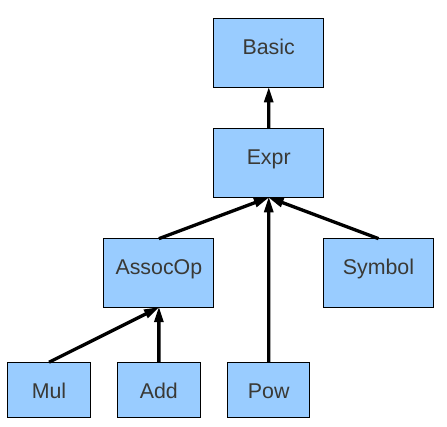
\includegraphics[scale=0.3]{../Pictures/sympyarch.png} 
\subsection{Variable et affection}\index{Variable et affection}

\begin{exercise}
Affectez les variables temps $t$ et distance $d$ par les valeurs 6.892 et 19.7. Calculez et affichez la valeur de la vitesse. Améliorez l'affichage en imposant un chiffre après le point décimal.
\end{exercise}

\begin{solution}
Pour, affectez des variables est les rendre symbolique comme c'est décrit dans le mémo ou il 
sera expliquer temps $t$ et distance $d$ par les valeurs 6.892 et 19.7. Calculez et affichez la 
valeur de la vitesse. Améliorez l'affichage en imposant un chiffre après le point décimal.
\end{solution}

\subsection{Contrôle du flux d’instructions}\index{Theorems!Single Line}
This is a theorem consisting of just one line.

\begin{exercise}
A set $\mathcal{D}(G)$ in dense in $L^2(G)$, $|\cdot|_0$. 
\end{exercise}
\begin{solution}
\end{solution}
%------------------------------------------------

\section{Les Fonctions}\index{Fonctions}

This is an example of a definition. A definition could be mathematical or it could define a concept.

\begin{exercise}
Écrire une fonction cube qui retourne le cube de son argument
\end{exercise}

\begin{exercise}
Écrire une fonction $volumeSphere$ qui calcule le volume d’une sphère de rayon $r$ fourni
en argument et qui utilise la fonction cube .
Tester la fonction $volumeSphere$ par un appel dans le programme principal.
\end{exercise}

\begin{exercise}
Écrire une fonction maFonction qui retourne $f(x) = 2x^{3} + x - 5$
\end{exercise}

\begin{exercise}
Écrire une fonction tabuler avec quatre paramètres : $fonction$ , $borneInf$ , $borneSup$
et $nbPas$ . Cette procédure affiche les valeurs de $fonction$ , de $borneInf$ à $borneSup$ ,
tous les nbPas . Elle doit respecter $borneInf < borneSup$.
Tester cette fonction par un appel dans le programme principal après avoir saisi les
deux bornes dans une floatbox et le nombre de pas dans une integerbox (utilisez le
module easyguiB ).
\end{exercise}

\begin{exercise}
Écrire une fonction $volMasse$ Ellipsoide qui retourne le volume et la masse d’un ellipsoïde grâce à un tuple. Les paramètres sont les trois demi-axes et la masse volumique. On donnera à ces quatre paramètres des valeurs par défaut. \\
On donne: $v = \frac{3}{4} \pi abc$ \\
Tester cette fonction par des appels avec différents nombres d’arguments.
\end{exercise}

\begin{exercise}
Une fonction $f (x)$ est lin\'eaire et a une valeur de $29$ \`a $x = -2$ et $39$ à $x = 3$. Trouver sa valeur à $x = 5$.
\end{exercise}

\begin{exercise}
Pour l'ensemble $N$ de nombres naturels et une opération binaire $f: N x N \longrightarrow N$, on appelle un élément $z$ $\epsilon$ $N$ une identité pour $f$, si $f (a, z) = a = f (z, a)$, pour tout a $\epsilon$ $N$. Lesquelles des opérations binaires suivantes ont une identité?:
\begin{enumerate}
  \item $f (x, y) = x + y - 3$
  \item $f (x, y) = max(x, y)$
  \item $f (x, y) = x^{y}$
\end{enumerate}
\end{exercise}
\begin{solution}
le deuxième et le troisième 
\end{solution}

